\documentclass[]{book}
\usepackage{lmodern}
\usepackage{amssymb,amsmath}
\usepackage{ifxetex,ifluatex}
\usepackage{fixltx2e} % provides \textsubscript
\ifnum 0\ifxetex 1\fi\ifluatex 1\fi=0 % if pdftex
  \usepackage[T1]{fontenc}
  \usepackage[utf8]{inputenc}
\else % if luatex or xelatex
  \ifxetex
    \usepackage{mathspec}
  \else
    \usepackage{fontspec}
  \fi
  \defaultfontfeatures{Ligatures=TeX,Scale=MatchLowercase}
\fi
% use upquote if available, for straight quotes in verbatim environments
\IfFileExists{upquote.sty}{\usepackage{upquote}}{}
% use microtype if available
\IfFileExists{microtype.sty}{%
\usepackage{microtype}
\UseMicrotypeSet[protrusion]{basicmath} % disable protrusion for tt fonts
}{}
\usepackage[margin=1in]{geometry}
\usepackage{hyperref}
\hypersetup{unicode=true,
            pdftitle={R로 배우는 기초통계},
            pdfauthor={한국생명공학연구원 김하성},
            pdfborder={0 0 0},
            breaklinks=true}
\urlstyle{same}  % don't use monospace font for urls
\usepackage{natbib}
\bibliographystyle{apalike}
\usepackage{color}
\usepackage{fancyvrb}
\newcommand{\VerbBar}{|}
\newcommand{\VERB}{\Verb[commandchars=\\\{\}]}
\DefineVerbatimEnvironment{Highlighting}{Verbatim}{commandchars=\\\{\}}
% Add ',fontsize=\small' for more characters per line
\usepackage{framed}
\definecolor{shadecolor}{RGB}{248,248,248}
\newenvironment{Shaded}{\begin{snugshade}}{\end{snugshade}}
\newcommand{\KeywordTok}[1]{\textcolor[rgb]{0.13,0.29,0.53}{\textbf{#1}}}
\newcommand{\DataTypeTok}[1]{\textcolor[rgb]{0.13,0.29,0.53}{#1}}
\newcommand{\DecValTok}[1]{\textcolor[rgb]{0.00,0.00,0.81}{#1}}
\newcommand{\BaseNTok}[1]{\textcolor[rgb]{0.00,0.00,0.81}{#1}}
\newcommand{\FloatTok}[1]{\textcolor[rgb]{0.00,0.00,0.81}{#1}}
\newcommand{\ConstantTok}[1]{\textcolor[rgb]{0.00,0.00,0.00}{#1}}
\newcommand{\CharTok}[1]{\textcolor[rgb]{0.31,0.60,0.02}{#1}}
\newcommand{\SpecialCharTok}[1]{\textcolor[rgb]{0.00,0.00,0.00}{#1}}
\newcommand{\StringTok}[1]{\textcolor[rgb]{0.31,0.60,0.02}{#1}}
\newcommand{\VerbatimStringTok}[1]{\textcolor[rgb]{0.31,0.60,0.02}{#1}}
\newcommand{\SpecialStringTok}[1]{\textcolor[rgb]{0.31,0.60,0.02}{#1}}
\newcommand{\ImportTok}[1]{#1}
\newcommand{\CommentTok}[1]{\textcolor[rgb]{0.56,0.35,0.01}{\textit{#1}}}
\newcommand{\DocumentationTok}[1]{\textcolor[rgb]{0.56,0.35,0.01}{\textbf{\textit{#1}}}}
\newcommand{\AnnotationTok}[1]{\textcolor[rgb]{0.56,0.35,0.01}{\textbf{\textit{#1}}}}
\newcommand{\CommentVarTok}[1]{\textcolor[rgb]{0.56,0.35,0.01}{\textbf{\textit{#1}}}}
\newcommand{\OtherTok}[1]{\textcolor[rgb]{0.56,0.35,0.01}{#1}}
\newcommand{\FunctionTok}[1]{\textcolor[rgb]{0.00,0.00,0.00}{#1}}
\newcommand{\VariableTok}[1]{\textcolor[rgb]{0.00,0.00,0.00}{#1}}
\newcommand{\ControlFlowTok}[1]{\textcolor[rgb]{0.13,0.29,0.53}{\textbf{#1}}}
\newcommand{\OperatorTok}[1]{\textcolor[rgb]{0.81,0.36,0.00}{\textbf{#1}}}
\newcommand{\BuiltInTok}[1]{#1}
\newcommand{\ExtensionTok}[1]{#1}
\newcommand{\PreprocessorTok}[1]{\textcolor[rgb]{0.56,0.35,0.01}{\textit{#1}}}
\newcommand{\AttributeTok}[1]{\textcolor[rgb]{0.77,0.63,0.00}{#1}}
\newcommand{\RegionMarkerTok}[1]{#1}
\newcommand{\InformationTok}[1]{\textcolor[rgb]{0.56,0.35,0.01}{\textbf{\textit{#1}}}}
\newcommand{\WarningTok}[1]{\textcolor[rgb]{0.56,0.35,0.01}{\textbf{\textit{#1}}}}
\newcommand{\AlertTok}[1]{\textcolor[rgb]{0.94,0.16,0.16}{#1}}
\newcommand{\ErrorTok}[1]{\textcolor[rgb]{0.64,0.00,0.00}{\textbf{#1}}}
\newcommand{\NormalTok}[1]{#1}
\usepackage{longtable,booktabs}
\usepackage{graphicx,grffile}
\makeatletter
\def\maxwidth{\ifdim\Gin@nat@width>\linewidth\linewidth\else\Gin@nat@width\fi}
\def\maxheight{\ifdim\Gin@nat@height>\textheight\textheight\else\Gin@nat@height\fi}
\makeatother
% Scale images if necessary, so that they will not overflow the page
% margins by default, and it is still possible to overwrite the defaults
% using explicit options in \includegraphics[width, height, ...]{}
\setkeys{Gin}{width=\maxwidth,height=\maxheight,keepaspectratio}
\IfFileExists{parskip.sty}{%
\usepackage{parskip}
}{% else
\setlength{\parindent}{0pt}
\setlength{\parskip}{6pt plus 2pt minus 1pt}
}
\setlength{\emergencystretch}{3em}  % prevent overfull lines
\providecommand{\tightlist}{%
  \setlength{\itemsep}{0pt}\setlength{\parskip}{0pt}}
\setcounter{secnumdepth}{5}
% Redefines (sub)paragraphs to behave more like sections
\ifx\paragraph\undefined\else
\let\oldparagraph\paragraph
\renewcommand{\paragraph}[1]{\oldparagraph{#1}\mbox{}}
\fi
\ifx\subparagraph\undefined\else
\let\oldsubparagraph\subparagraph
\renewcommand{\subparagraph}[1]{\oldsubparagraph{#1}\mbox{}}
\fi

%%% Use protect on footnotes to avoid problems with footnotes in titles
\let\rmarkdownfootnote\footnote%
\def\footnote{\protect\rmarkdownfootnote}

%%% Change title format to be more compact
\usepackage{titling}

% Create subtitle command for use in maketitle
\providecommand{\subtitle}[1]{
  \posttitle{
    \begin{center}\large#1\end{center}
    }
}

\setlength{\droptitle}{-2em}

  \title{R로 배우는 기초통계}
    \pretitle{\vspace{\droptitle}\centering\huge}
  \posttitle{\par}
    \author{한국생명공학연구원 김하성}
    \preauthor{\centering\large\emph}
  \postauthor{\par}
      \predate{\centering\large\emph}
  \postdate{\par}
    \date{2019-09-03}

\usepackage{booktabs}
\usepackage{amsthm}
\makeatletter
\def\thm@space@setup{%
  \thm@preskip=8pt plus 2pt minus 4pt
  \thm@postskip=\thm@preskip
}
\makeatother

\begin{document}
\maketitle

{
\setcounter{tocdepth}{1}
\tableofcontents
}
\hypertarget{lecture-}{%
\chapter{Lecture 개요}\label{lecture-}}

\begin{itemize}
\tightlist
\item
  장소: 한국생명공학연구원 연구동 세미나실 1213호 (매주수요일 13:00\textasciitilde{}16:00)
\item
  강사: 한국생명공학연구원 바이오합성연구센터 김하성
\item
  연락처: 042-860-4372, \href{mailto:haseong@kribb.re.kr}{\nolinkurl{haseong@kribb.re.kr}} (생명연 연구동 1143)
\item
  강의site: \url{https://greendaygh.github.io/Rstat2019/}
\end{itemize}

\hypertarget{goal--}{%
\section{Goal 강의 목표}\label{goal--}}

\begin{itemize}
\tightlist
\item
  이공계열 대학원생이 보다 쉽게 통계 이론을 습득하고 활용하는 능력을 배양하는데 주요 목적이 있음. 특히 데이터 분석용 프로그래밍언어인 R을 기반으로 한 실습을 통하여 프로그래밍 기술 습득과 함께 데이터를 다루는 능력을 배움으로써 이공계 연구에 있어서 필수인 통계적 사고의 기초를 다지는데 그 목적이 있음.
\end{itemize}

\hypertarget{references--}{%
\section{References 참고 자료}\label{references--}}

\begin{itemize}
\tightlist
\item
  Using R for Introductory Statistics by John Verzani

  \begin{itemize}
  \tightlist
  \item
    Free version of 1st Edition

    \begin{itemize}
    \tightlist
    \item
      \url{https://cran.r-project.org/doc/contrib/Verzani-SimpleR.pdf}
    \item
      \url{http://cbb.sjtu.edu.cn/~mywu/bi217/usingR.pdf}
    \end{itemize}
  \item
    Second edition

    \begin{itemize}
    \tightlist
    \item
      \url{https://www.crcpress.com/Using-R-for-Introductory-Statistics-Second-Edition/Verzani/p/book/9781466590731}
    \end{itemize}
  \end{itemize}
\item
  R for Data Science (\url{https://r4ds.had.co.nz}, \url{https://github.com/hadley})
\item
  \url{https://resources.rstudio.com/}
\item
  일반통계학 (영지문화사, 김우철 외)
\end{itemize}

\hypertarget{evaluation---}{%
\section{Evaluation 평가 세부 항목}\label{evaluation---}}

\begin{itemize}
\tightlist
\item
  출석 50\% / 과제 50\% / 80점 이상 S, 80점 미만 U 부여
\end{itemize}

\hypertarget{schedule--}{%
\section{Schedule 강의 계획}\label{schedule--}}

\begin{itemize}
\item
  1주차- R basics / introduction of data
\item
  2주차 - Univariate data -- Summary statistics 일변량자료 (범주형, 수치형, 분포)
\item
  3주차 - Bivariate data -- Correlation / Independence 이변량자료 (자료비교, 수치자료의 관계, 단순선형회귀)
\item
  4주차 - Multivariate data -- R data structure 다변량자료 (다변량, R자료형, R그래픽)
\item
  5주차 - Populations -- Families of distributions 모집단과 분포
\item
  6주차 - Sampling -- Distribution and CLT 시뮬레이션, 샘플링
\item
  7주차 - Statistical inference 통계적 추론
\item
  8주차 - Confidence intervals 신뢰구간
\item
  9주차 - Significance test - parameteric 유의성 검정 (모수)
\item
  10주차 - Significance test -- non parametric 유의성 검정 (비모수)
\item
  11주차 - Goodness of fit - parametric 적합도 검정 (모수)
\item
  12주차 - Goodness of fit -- non parametirc 적합도 검정 (비모수)
\item
  13주차 - Linear regression -- basics \& simple LR 단순회귀모형
\item
  14주차 - Multiple linear regression 다중회귀모형
\item
  15주차 - Analysis of variance 분산분석
\item
  16주차 - Logistic / Non-linear regression 로지스틱/비선형회귀모형
\item
  9/25 휴강 (강사 해외 출장)
\end{itemize}

\hypertarget{references---1}{%
\section{References 참고 자료}\label{references---1}}

\begin{itemize}
\tightlist
\item
  R 홈페이지 \url{https://www.r-project.org/}
\item
  Rstudio 홈페이지 \url{https://www.rstudio.com/}
\item
  Packages for biologists \url{https://www.bioconductor.org/}
\item
  R 기본 문서들 (소개, 사용, 설치, 운영)
\item
  \url{https://cran.r-project.org/doc/manuals/r-release/R-intro.html}
\item
  \url{https://cran.r-project.org/doc/manuals/r-release/R-data.html}
\item
  \url{https://cran.r-project.org/doc/manuals/r-release/R-admin.html}
\item
  R ebooks
\item
  \url{https://bookdown.org/}
\end{itemize}

\hypertarget{introductin-}{%
\chapter{Introductin 개요}\label{introductin-}}

\hypertarget{what-is-r-rstudio}{%
\section{What is R / Rstudio}\label{what-is-r-rstudio}}


\includegraphics{images/r.jpg}

\begin{itemize}
\tightlist
\item
  R is a programming language that runs computations (\url{https://www.r-project.org/})
\item
  RStudio is an integrated development environment (IDE) that provides an interface for the programming (\url{https://www.rstudio.com/})
\end{itemize}

\hypertarget{r-rstudio-installation}{%
\section{R / Rstudio installation}\label{r-rstudio-installation}}

\begin{itemize}
\item
  Install R first and then install RStudio second
\item
  R
  
\includegraphics{images/01-01.PNG}\\
  
\includegraphics{images/01-02.PNG}\\
  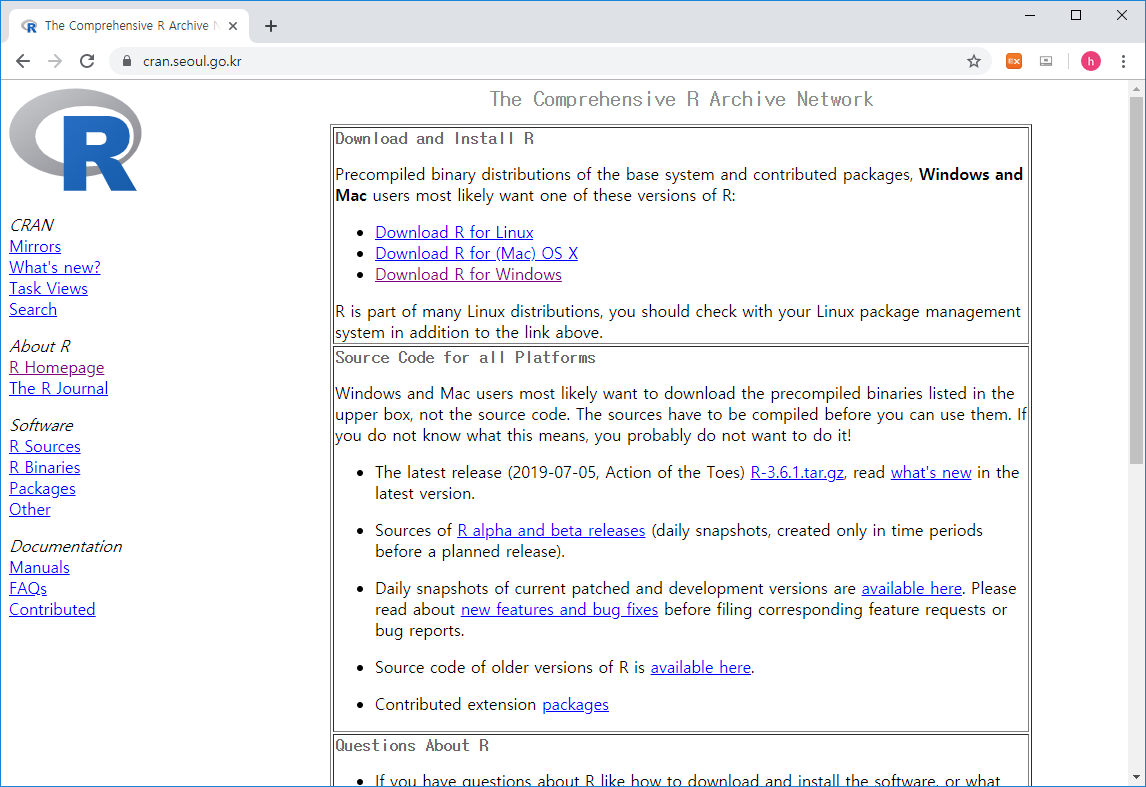
\includegraphics{images/01-03.PNG}\\
  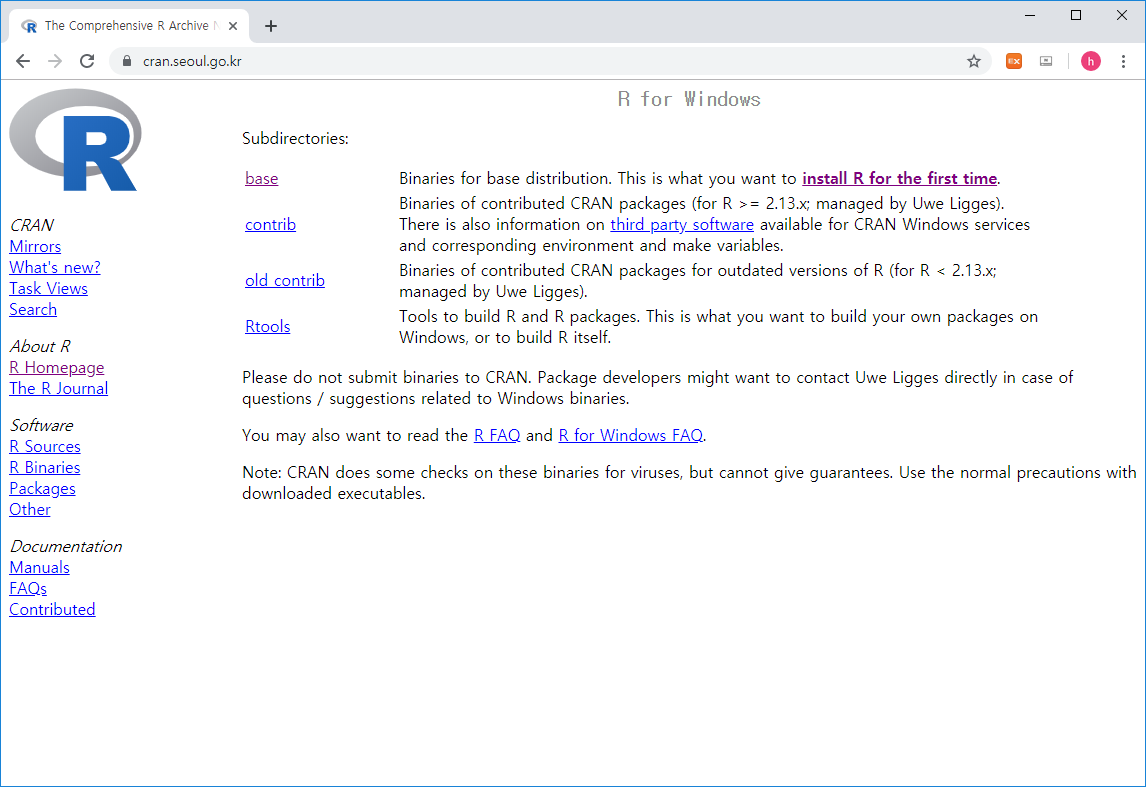
\includegraphics{images/01-04.PNG}\\
  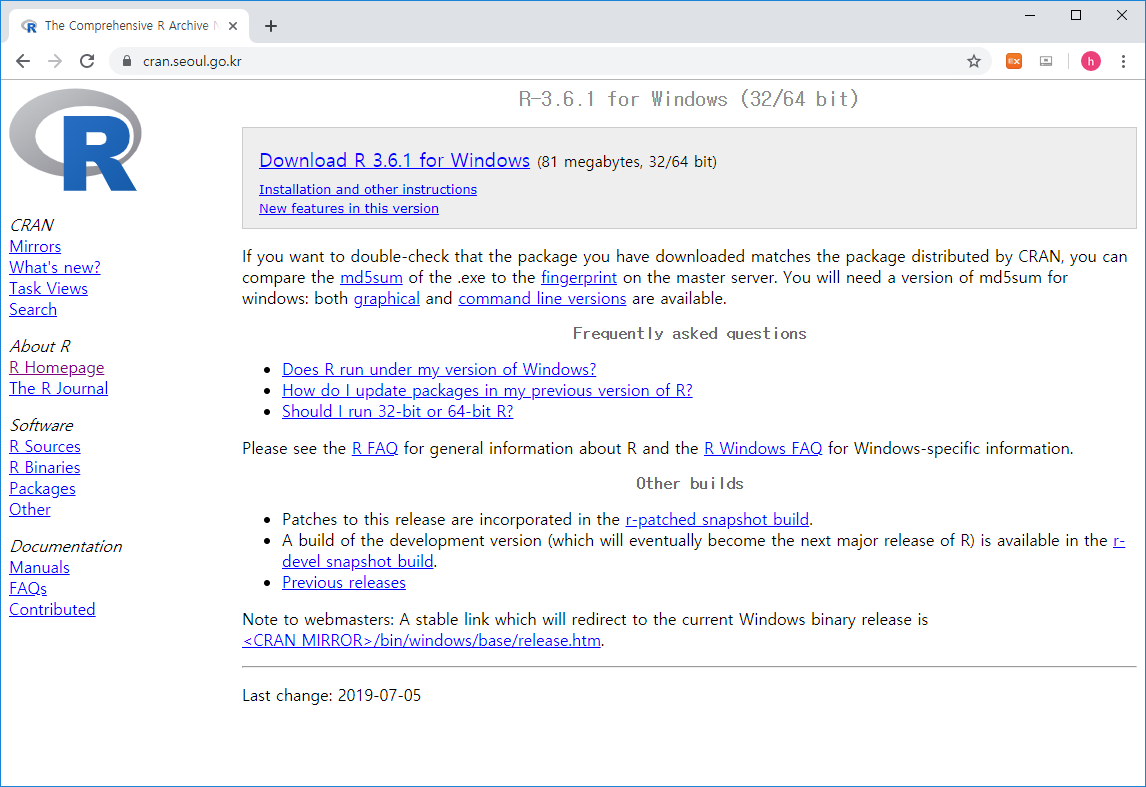
\includegraphics{images/01-05.PNG}
\item
  Rstudio
  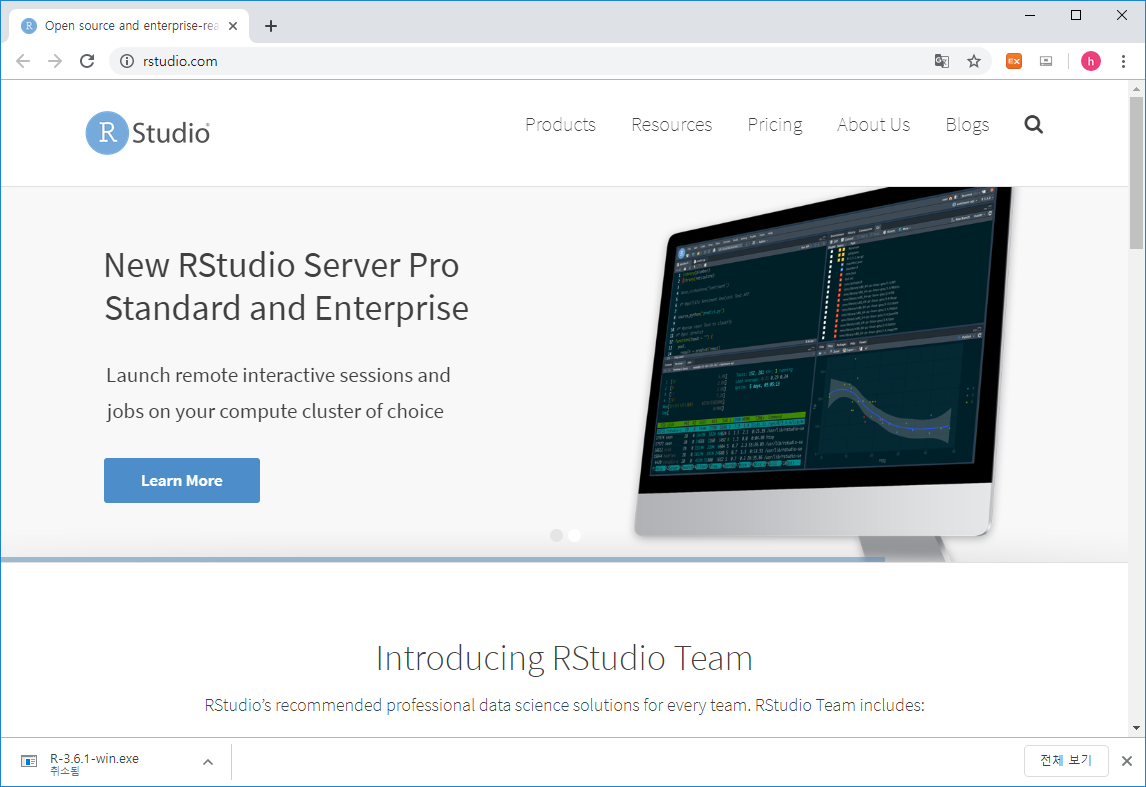
\includegraphics{images/01-06.PNG}\\
  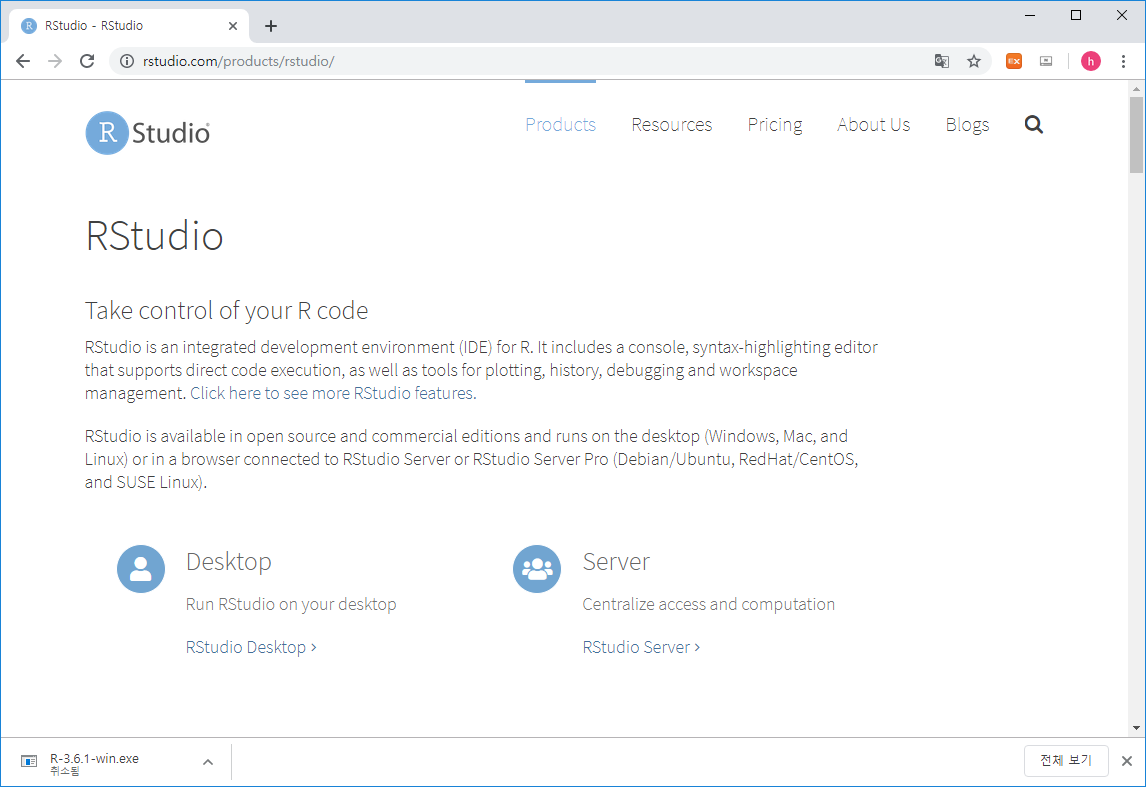
\includegraphics{images/01-07.PNG}\\
  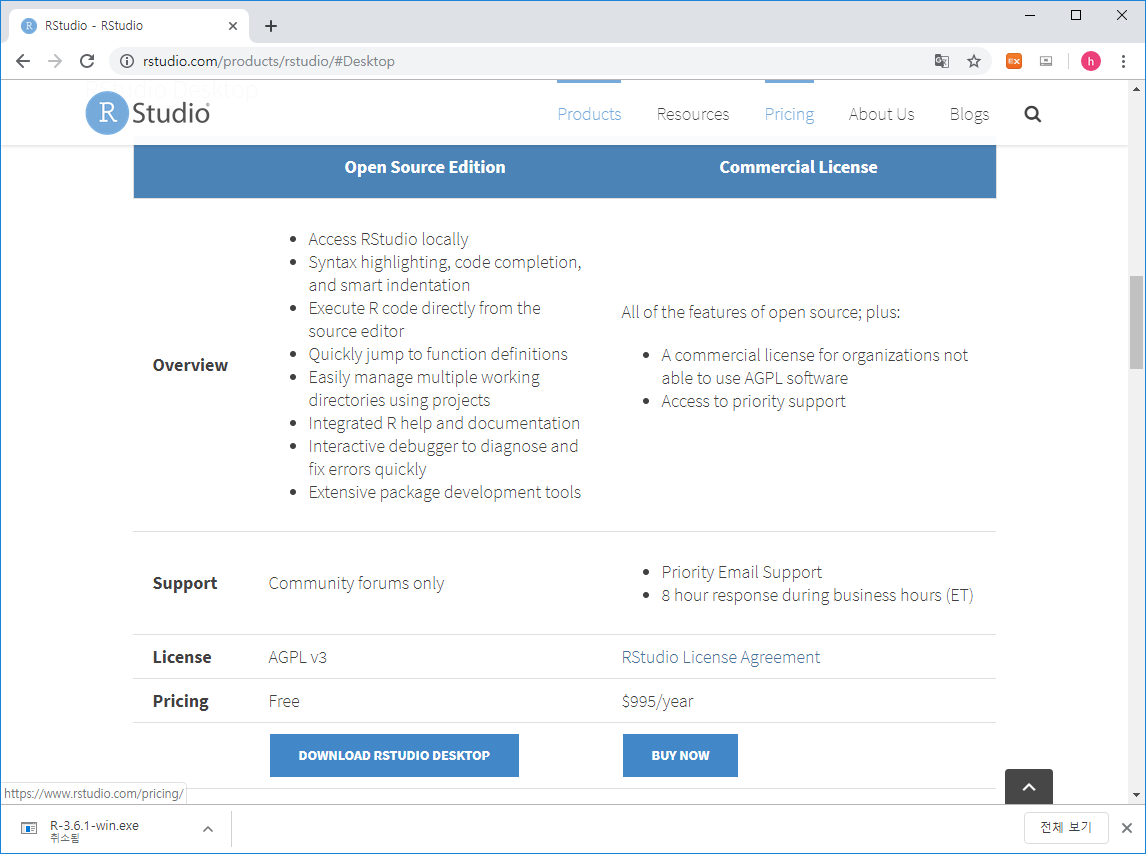
\includegraphics{images/01-08.PNG}\\
  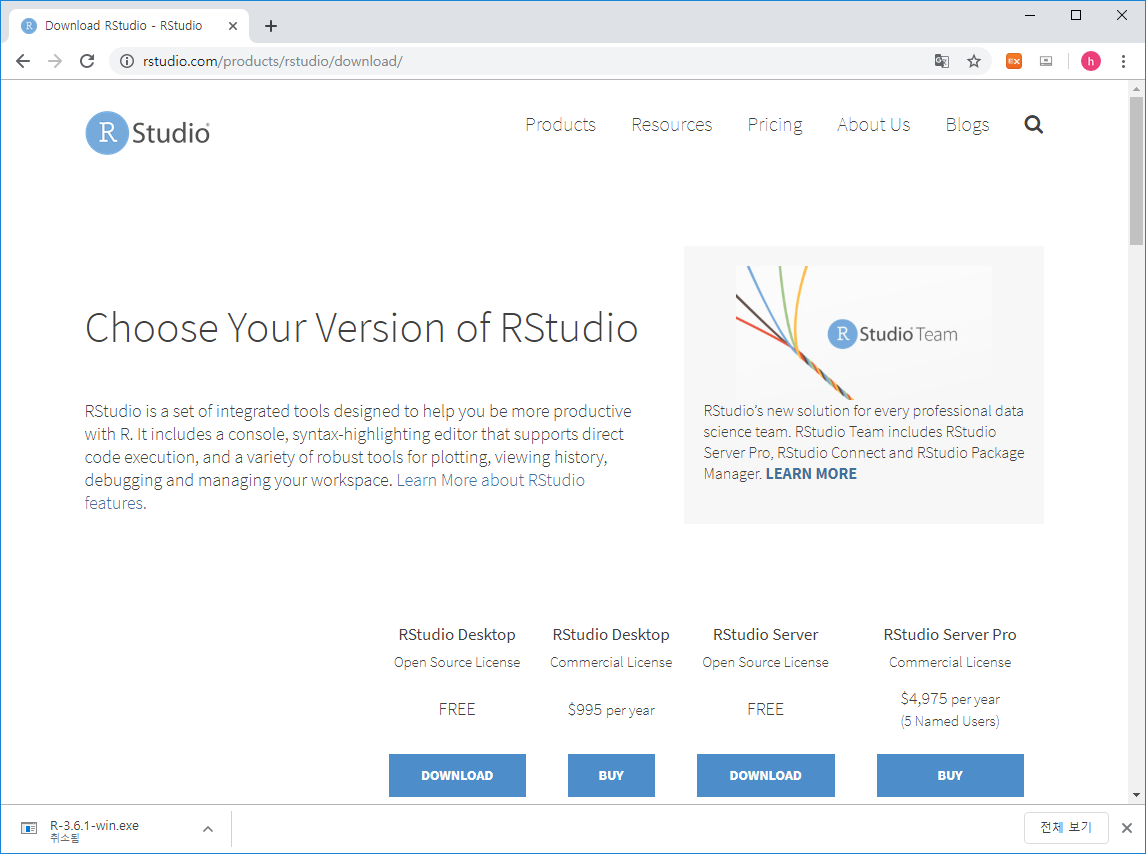
\includegraphics{images/01-09.PNG}\\
  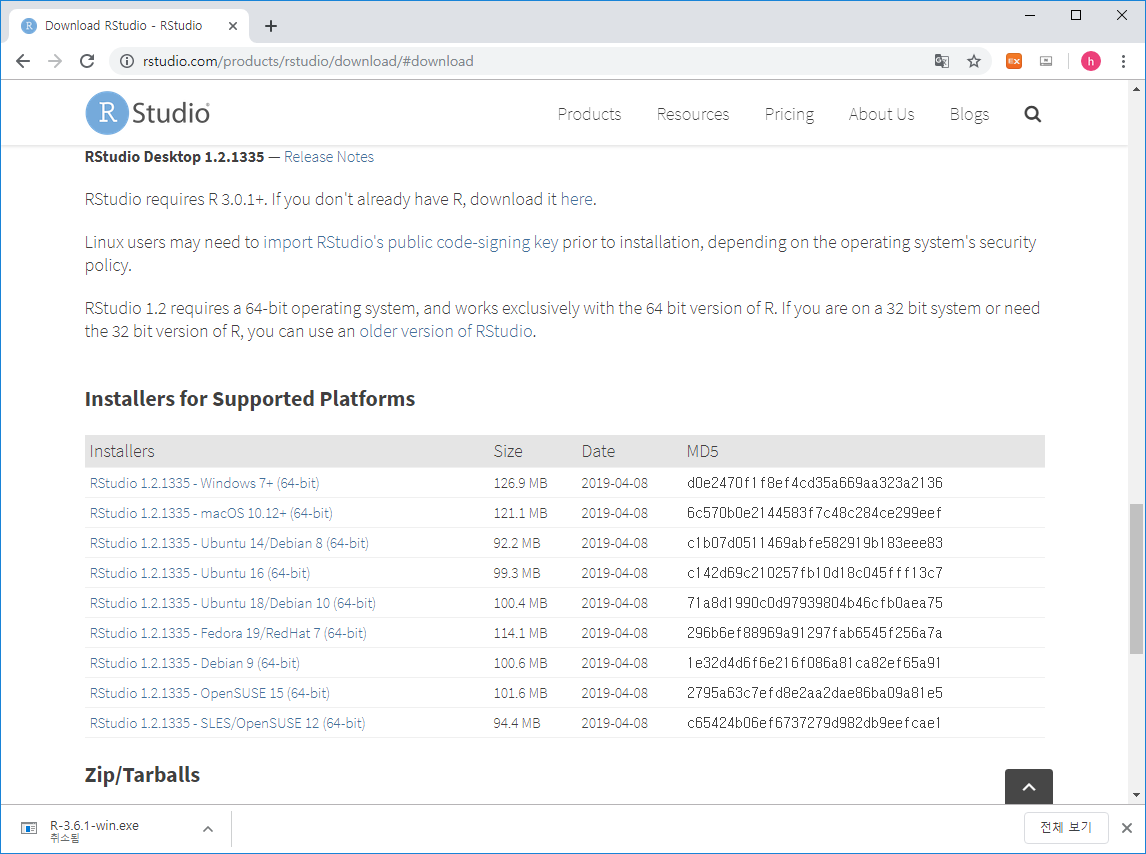
\includegraphics{images/01-10.PNG}
\end{itemize}

\hypertarget{rstudio-interface}{%
\section{Rstudio interface}\label{rstudio-interface}}

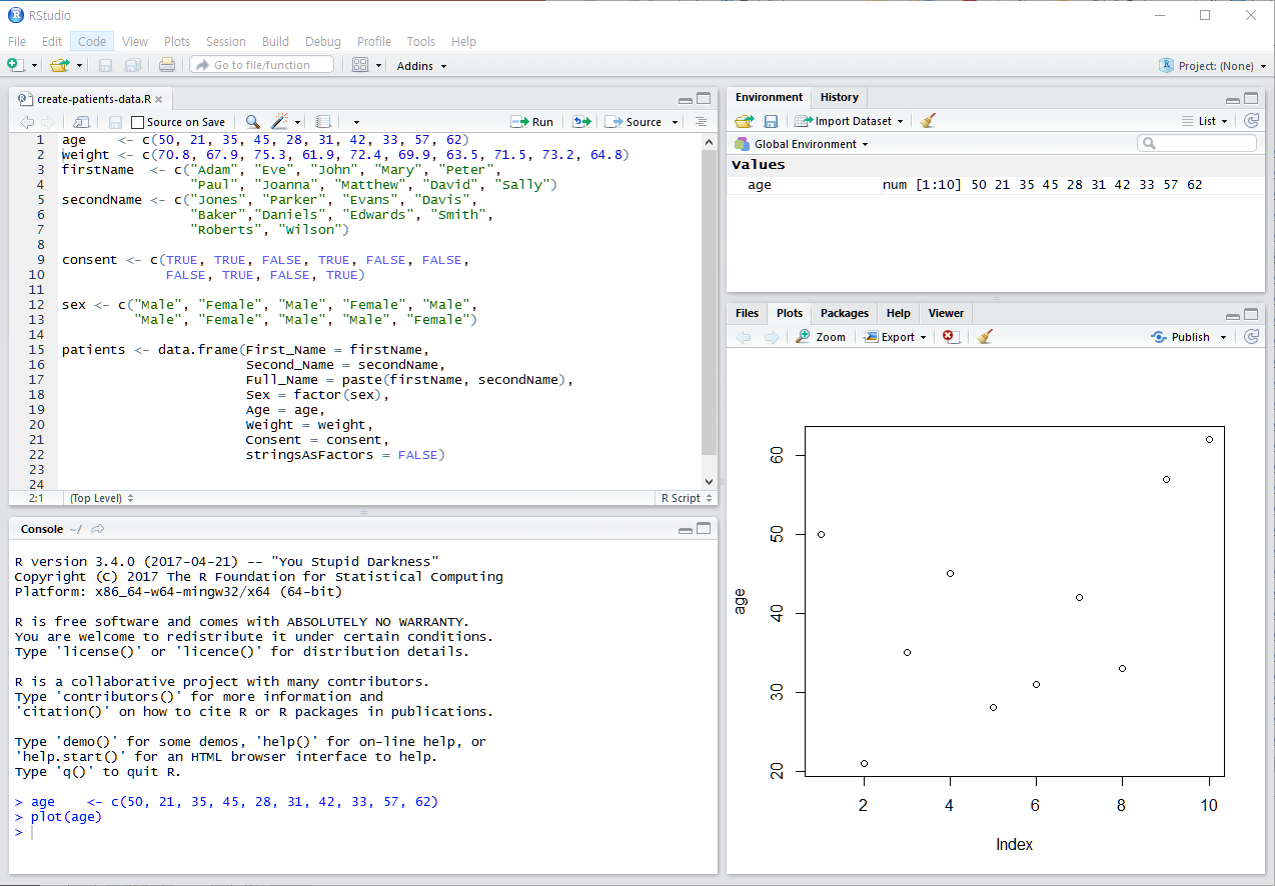
\includegraphics{images/01-11.PNG}

\hypertarget{r-code-basics}{%
\section{R code basics}\label{r-code-basics}}

\begin{itemize}
\tightlist
\item
  Basics:
  Console: Where you enter in commands.
  Running code: The act of telling R to perform an act by giving it commands in the console.
  Objects: Where values are saved in R. We'll show you how to assign values to objects and how to display the contents of objects.
  Data types: Integers, doubles/numerics, logicals, and characters.
  Vectors: A series of values. These are created using the c() function, where c() stands for ``combine'' or ``concatenate.'' For example: c(6, 11, 13, 31, 90, 92).
  Factors: Categorical data are represented in R as factors.
  Data frames: Data frames are like rectangular spreadsheets: they are representations of datasets in R where the rows correspond to observations and the columns correspond to variables that describe the observations. We'll cover data frames later in Section 1.4.
  Conditionals:
  Testing for equality in R using == (and not = which is typically used for assignment). Ex: 2 + 1 == 3 compares 2 + 1 to 3 and is correct R code, while 2 + 1 = 3 will return an error.
  Boolean algebra: TRUE/FALSE statements and mathematical operators such as \textless{} (less than), \textless{}= (less than or equal), and != (not equal to).
  Logical operators: \& representing ``and'' as well as \textbar{} representing ``or.'' Ex: (2 + 1 == 3) \& (2 + 1 == 4) returns FALSE since both clauses are not TRUE (only the first clause is TRUE). On the other hand, (2 + 1 == 3) \textbar{} (2 + 1 == 4) returns TRUE since at least one of the two clauses is TRUE.
  Functions, also called commands: Functions perform tasks in R. They take in inputs called arguments and return outputs. You can either manually specify a function's arguments or use the function's default values.
\end{itemize}

\hypertarget{introduction-of-data}{%
\chapter{introduction of data}\label{introduction-of-data}}

You can label chapter and section titles using \texttt{\{\#label\}} after them, e.g., we can reference Chapter \ref{intro}. If you do not manually label them, there will be automatic labels anyway, e.g., Chapter \ref{methods}.

Figures and tables with captions will be placed in \texttt{figure} and \texttt{table} environments, respectively.

\begin{Shaded}
\begin{Highlighting}[]
\KeywordTok{par}\NormalTok{(}\DataTypeTok{mar =} \KeywordTok{c}\NormalTok{(}\DecValTok{4}\NormalTok{, }\DecValTok{4}\NormalTok{, }\FloatTok{.1}\NormalTok{, }\FloatTok{.1}\NormalTok{))}
\KeywordTok{plot}\NormalTok{(pressure, }\DataTypeTok{type =} \StringTok{'b'}\NormalTok{, }\DataTypeTok{pch =} \DecValTok{19}\NormalTok{)}
\end{Highlighting}
\end{Shaded}

\begin{figure}

{\centering 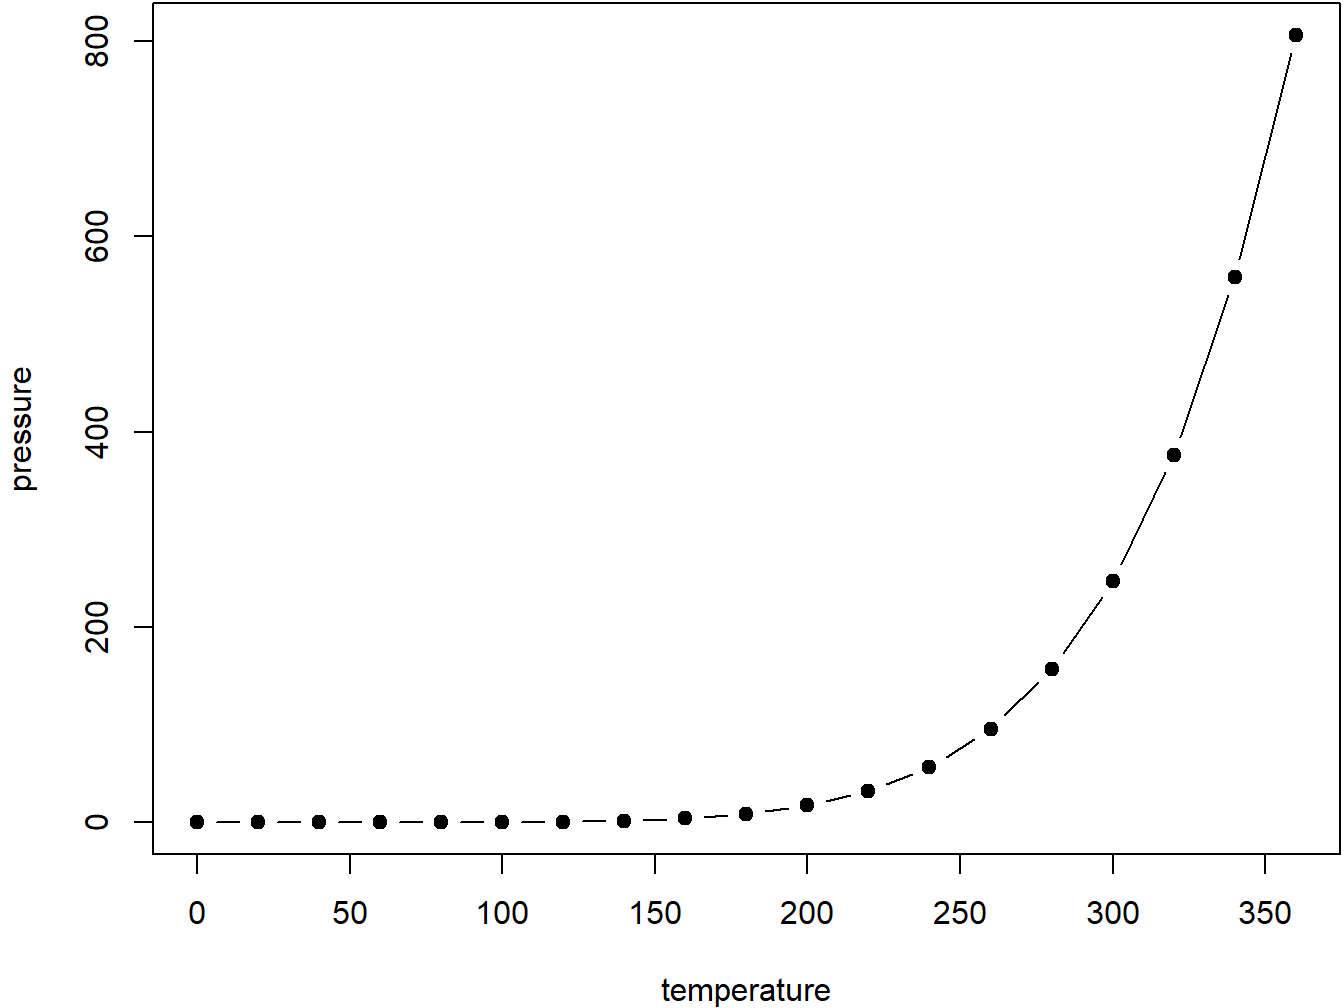
\includegraphics[width=0.8\linewidth]{Rstat_files/figure-latex/nice-fig-1} 

}

\caption{Here is a nice figure!}\label{fig:nice-fig}
\end{figure}

Reference a figure by its code chunk label with the \texttt{fig:} prefix, e.g., see Figure \ref{fig:nice-fig}. Similarly, you can reference tables generated from \texttt{knitr::kable()}, e.g., see Table \ref{tab:nice-tab}.

\begin{Shaded}
\begin{Highlighting}[]
\NormalTok{knitr}\OperatorTok{::}\KeywordTok{kable}\NormalTok{(}
  \KeywordTok{head}\NormalTok{(iris, }\DecValTok{20}\NormalTok{), }\DataTypeTok{caption =} \StringTok{'Here is a nice table!'}\NormalTok{,}
  \DataTypeTok{booktabs =} \OtherTok{TRUE}
\NormalTok{)}
\end{Highlighting}
\end{Shaded}

\begin{table}[t]

\caption{\label{tab:nice-tab}Here is a nice table!}
\centering
\begin{tabular}{rrrrl}
\toprule
Sepal.Length & Sepal.Width & Petal.Length & Petal.Width & Species\\
\midrule
5.1 & 3.5 & 1.4 & 0.2 & setosa\\
4.9 & 3.0 & 1.4 & 0.2 & setosa\\
4.7 & 3.2 & 1.3 & 0.2 & setosa\\
4.6 & 3.1 & 1.5 & 0.2 & setosa\\
5.0 & 3.6 & 1.4 & 0.2 & setosa\\
\addlinespace
5.4 & 3.9 & 1.7 & 0.4 & setosa\\
4.6 & 3.4 & 1.4 & 0.3 & setosa\\
5.0 & 3.4 & 1.5 & 0.2 & setosa\\
4.4 & 2.9 & 1.4 & 0.2 & setosa\\
4.9 & 3.1 & 1.5 & 0.1 & setosa\\
\addlinespace
5.4 & 3.7 & 1.5 & 0.2 & setosa\\
4.8 & 3.4 & 1.6 & 0.2 & setosa\\
4.8 & 3.0 & 1.4 & 0.1 & setosa\\
4.3 & 3.0 & 1.1 & 0.1 & setosa\\
5.8 & 4.0 & 1.2 & 0.2 & setosa\\
\addlinespace
5.7 & 4.4 & 1.5 & 0.4 & setosa\\
5.4 & 3.9 & 1.3 & 0.4 & setosa\\
5.1 & 3.5 & 1.4 & 0.3 & setosa\\
5.7 & 3.8 & 1.7 & 0.3 & setosa\\
5.1 & 3.8 & 1.5 & 0.3 & setosa\\
\bottomrule
\end{tabular}
\end{table}

You can write citations, too. For example, we are using the \textbf{bookdown} package \citep{R-bookdown} in this sample book, which was built on top of R Markdown and \textbf{knitr} \citep{xie2015}.

\bibliography{book.bib,packages.bib}


\end{document}
